\chapter{Quantum Dynamics} 
\label{ch:QuantumDynamics}

\section{Closed Quantum Systems}

We begin by quickly summarising the laws of quantum mechanics as applied to a \textit{closed system}; that is, a system which does not interact in any way with other systems. In practice, it is rare that any given system can truly be considered to be closed, yet the dynamics of closed systems are fundamental to the quantum mechanical description of nature: at the highest level, we can view the universe itself an closed quantum system which contains all others.

By considering idealised closed systems, we are able to present the purest form of the rules of quantum mechanics: three postulates concerning the system's state, its evolution, and the act of performing measurements on it. In the latter part of this chapter we will generalise the laws stated here to address \textit{open systems}, by first considering the open system as part of a larger closed system to which the postulates apply.

\subsection{State}

The first postulate concerns the description of the state of a system~\cite{nielsen+chuang}:
\begin{quotation}
  Associated to any closed physical system is a Hilbert space known as the \textit{state space} of the system. The system is completely described by its \textit{state vector}, which is a unit vector in the system's state space. The state space of a composite physical system is the tensor product of the state spaces of the component physical systems.
\end{quotation}
A Hilbert space is a (possibly infinite-dimensional) vector space over the complex numbers, on which an inner product is defined. Note that the postulate does not specify how the correct state space for a given system should be chosen, which is therefore a judgment that must be made when the system is modelled.

In general, when a system can be described using a state vector we say that it exists in a \textit{pure state}. With the state vector specified we have complete knowledge about the system - we know everything that there is to know. We will usually write the state vector using the Dirac bracket notation, $\ket{\psi}$. 

In QIP we are often concerned with physical systems where the state space is two-dimensional: the quantum bit or \textit{qubit}. The general state of such as system can be written
\begin{align}
  \ket{\psi} = \alpha\ket{0} + \beta\ket{1}
\end{align}
where the normalisation condition is imposed by requiring that $|\alpha|^2 + |\beta|^2 = 1$. As an alternative representation we can write
\begin{align}
  \ket{\psi} = \cos\frac{\theta}{2}\ket{0} + e^{i\phi}\sin\frac{\theta}{2}\ket{1}
\end{align}
where we have used the fact that two states are physically equivalent if they differ by a global phase, $\ket{a} = e^{ik}\ket{b}$, which will become apparent when we look at the measurement postulate. We can use this representation to visualise a qubit as a point on the surface of a unit sphere, known as the \textit{Bloch sphere}, described by the real $3$-vector $(\cos\phi\sin\theta, \sin\phi\sin\theta, \cos\theta)$ (Fig.~\ref{bloch_sphere}).

\begin{figure}[htb]
  \begin{center}
    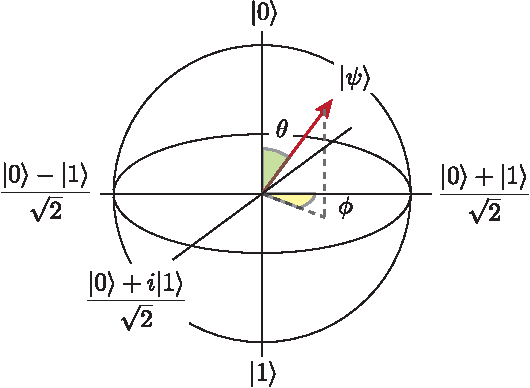
\includegraphics{figures/bloch_sphere.pdf}
  \end{center}
  \caption{The Bloch Sphere: the state $\ket{\psi} =  \cos\frac{\theta}{2}\ket{0} + e^{i\phi}\sin\frac{\theta}{2}\ket{1}$ is represented as a vector pointing to a point on a unit sphere, with spherical polar coordinates $(\theta, \phi)$. }
  \label{bloch_sphere}
\end{figure}

\subsection{Dynamics}

The second postulate concerns the evolution of an isolated quantum system and can be stated~\cite{nielsen+chuang}:
\begin{quotation}
The time evolution of an isolated quantum system is described by the \textit{Schr\"odinger equation},
\begin{align}
  \label{qd:schrodinger_eq}
  i\hbar\ddt \ket{\psi(t)} = H(t) \ket{\psi(t)}
\end{align}
where $\hbar$ is a constant, known as \textit{Planck's constant}, and $H(t)$ is a fixed Hermitian operator known as the Hamiltonian of the closed system.
\end{quotation}
In the rest of this thesis we choose units so as to set $\hbar = 1$, unless stated otherwise. 

The Schr\"odinger equation can be solved in terms of a time evolution operator
\begin{align}
  \ket{\psi(t)} = U(t)\ket{\psi(0)}
\end{align}
where $U(t)$ is the solution to the differential equation
\begin{align}
  \ddt U(t) = H(t)U(t), \qquad U(0) = \id
\end{align}
As $H(t)$ is Hermitian, $U(t)$ will be unitary. In particular this implies that $U^{-1}(t) = U^\dagger(t)$, so the inverse of $U(t)$ exists and therefore the dynamics of isolated quantum systems are reversible.

As the Hamiltonian is Hermitian we can write it in the form
\begin{align}
  H = \sum_i E_i \ket{\phi_i}\bra{\phi_i}
\end{align}
where $E_i$ are the eigenvalues, which are real, and $\ket{\phi_i}$ are the associated eigenvectors, which can be chosen to be orthogonal. The $\ket{\phi_i}$ are sometimes called stationary states, as they evolve as
\begin{align}
  \ket{\phi_i(t)} = e^{-i E_i t}\ket{\phi_i(0)}
\end{align}
picking up a phase at rate $E_i$.

As a simple example of pure state evolution we consider an isolated qubit, under the influence of the \textit{Rabi Hamiltonian},
\begin{equation} \label{rabi_hamiltonian}
  H = \frac{1}{2}
\begin{bmatrix}
  -\nu & \Omega \\
  \Omega & \nu 
\end{bmatrix},
\end{equation}
in the $\{\ket{0}, \ket{1}\}$ basis. We diagonalise the Hamiltonian
\begin{align}
  H = E_1 \ket{\phi_1}\bra{\phi_1} + E_2 \ket{\phi_2}\bra{\phi_2}
\end{align}
in terms of the eigenvectors and eigenvalues
\begin{align}
  \ket{\phi_1} &=  \cos\frac{\theta}{2}\ket{0} + \sin\frac{\theta}{2}\ket{1}  &E_1 = \nu + \sqrt{\nu^2 + \Omega^2} \\
  \ket{\phi_2} &=  \sin\frac{\theta}{2}\ket{0} + \cos\frac{\theta}{2}\ket{1} &E_2 = \nu - \sqrt{\nu^2 + \Omega^2} 
\end{align}
where
\begin{align}
  \theta = \arctan\left(\frac{\Omega}{\nu}\right).
\end{align}

We can then write the solution to the Schr\"odinger equation
\begin{align}
  \ket{\psi(t)} &= \alpha e^{iE_1t}\ket{\phi_1} +  \beta e^{iE_2t} \ket{\phi_2} \\
  &= \alpha e^{i\Delta t}\ket{\phi_1} +  \beta e^{- i\Delta t} \ket{\phi_2} 
\end{align}
where $\Delta = \sqrt{\nu^2 + \Omega^2}$, $\alpha$ and $\beta$ are constants, and the last equality uses the equivalence of two quantum states differing only by a global phase. 

The solution can be visualised as rotation of the initial state vector about the axis connecting the diametrically opposite points relating $\ket{\phi_1}$ and $\ket{\phi_2}$ on the Bloch sphere, at angular speed $\Delta$. The amplitude of the oscillation is proportional to $\sin^2\theta$, increasing from $0$ to $1$ as $\theta \rightarrow \pi$.  This oscillatory behaviour, known in this case as the \textit{Rabi oscillation}, is a common feature of many quantum systems.

\subsection{Measurements}

The third, and final, postulate concerns itself with measurements performed on isolated quantum systems. We state it in terms of a special class of measurements~\cite{nielsen+chuang}:
\begin{quotation}
  A \textit{projective measurement} is described by an \textit{observable}, M, a Hermitian operator on the system's state space. We can write the operator as
  \begin{align}
    M = \sum_m mP_m
  \end{align}
  where $P_m$ is the projector onto the eigenspace of $M$ with eigenvalue $m$. The outcomes of the measurement correspond to the eigenvalues $m$. When performing a measurement on state $\ket{\psi}$, the probability of obtaining outcome $m$ is
  \begin{align}
    p(m) = \bra{\psi}P_m\ket{\psi}.
  \end{align}
  Given that outcome $m$ occurred, the state of the system immediately after the measurement is
  \begin{align}
    \frac{P_m\ket{\psi}}{\sqrt{p(m)}}.
  \end{align}
\end{quotation}
In fact, projective measurements are not the most general measurement we can make on a closed quantum system. A projective measurement corresponds to making a measurement on the whole system. We could also choose to just measure a part of the system, which would not generally perform a projective measurement on the whole. We state postulate three in terms of projective measurements as they are conceptually simple and it can be shown that the most general types of measurements are always equivalent to a projective measurement on some ancilliary system \cite{peres}. We visit these more general measurements along with open quantum systems in the next section.


\section{Open Quantum Systems}

In reality, a closed quantum system must be viewed as an idealisation; with the possible exception of the entire universe, the assumption that a system is closed must always be approximate as all physical systems are unavoidably coupled to other physical systems. We could try to rectify the situation by expanding the system we are interested in to include these other systems, but will eventually run into difficulties: when considered together the joint system may be too complex to model given our computational resources, or perhaps we do not have enough knowledge of some of the systems or couplings to make modelling possible. To model real-world situations we must develop the theory of \textit{open quantum systems}. 

The subject of open quantum systems is especially important for the field of QIP. Most QIP processes and algorithms are stated in terms of what can be done in principle in ideal systems. All real systems suffer from unwanted interactions with other systems. In assessing a system's suitability as a candidate QIP system, it is important to be able to somehow incorporate these interactions into our model and evaluate the extent of their effect on the system's information processing capacity.

In order to treat open systems we will need to generalise the ideas of state description, evolution and measurement that were introduced in the previous section.



\subsection{State}

When describing the state of closed systems we used the state vector. The state vector represents complete knowledge of the system. When we deal with open quantum systems, we frequently find ourselves in situations where we do not have this complete knowledge - there is some classical uncertainty in our knowledge of the state. In these cases the state vector is no longer sufficient for giving the best possible representation of the state. 

As a simple illustration of this point, consider a pair of qubits in the Bell singlet state, $(\ket{01} - \ket{10})/\sqrt{2}$. Imagine we only have access to the first qubit and want to provide the best possible description of its state; another party holds the second qubit and there are no restrictions placed on the operations they perform. A first observation is that if we perform a projective measurement described by the $Z$ operator we obtain the outcomes $0$ and $1$, each with probability $1/2$. The only state vectors with this property take the form $(\ket{0} + e^{i\phi}\ket{1})/\sqrt{2}$, with $\phi \in [0, 2\pi)$. However, our first qubit also has the property that when measured in the $X$ or $Y$ basis it will also report both possible outcomes with equal probability, which is not the case for any of the state vectors given. A good representation of the state of the first qubit is not possible within the language of state vectors.

Systems where the state is not completely known, and subsystems of composite systems, can be thought of as being in a statistical mixture of pure states. We say these systems exist in a \textit{mixed state}. To describe such states, we introduce the \textit{density matrix}
\begin{align}
  \rho = \sum_i p_i \ket{\psi_i}\bra{\psi_i},
\end{align}
which represents a statistical mixture of pure states $\ket{\psi_i}$ each with probability $p_i$. It can be seen immediately that a density matrix must be Hermitian and positive semi-definite (has all eigenvalues $\geq 0$), and that $\tr(\rho) = 1$. It is also true that any matrix satisfying these properties will describe the state of some quantum ensemble.

When we introduced the concept of a mixed state we did not rule out that the state is also pure, merely that it need not be. We can consider a pure state to be a statistical `mixture' of a single state:
\begin{align}
  \rho = \ket{\psi}\bra{\psi}.
\end{align}
Pure states can be identified by the fact that $\tr\{\rho^2\} = 1$. In general $\tr\{\rho^2\}$ can be used as a measure of how pure a state is. A maximally mixed state in a Hilbert space of dimension $n$ has $\rho = \id_n/n$ and $\tr\{\rho^2\} = 1/n$.

If we have a composite quantum system formed from two systems $A$ and $B$ the density matrix of the joint system is given
\begin{align}
  \rho_{AB} = \rho_A \otimes \rho_B. 
\end{align}
If we are given the density matrix of the joint system, we can find the reduced density matrix of the subsystem $A$ by taking the \textit{partial trace} over $B$,
\begin{align}
  \rho_A = \tr_B\{\rho_{AB}\} = \sum_b \bra{b}\rho_{AB}\ket{b},
\end{align}
where $\{\ket{b}\}$ is a basis for the Hilbert space of system $B$. 

\subsection{Measurement}

We earlier stated the measurement postulate in terms of projective measurements: a measurement on an isolated quantum system is described by a single operator and the possible measurement outcomes are given by the eigenvalues of that operator. The act of measurement projects the system into the eigenspace of the eigenvalue corresponding to the outcome. 

When dealing with non-isolated systems we must extend our measurement framework to \textit{positive operator valued measurements} (POVMs). Neumark's theorem \cite{peres} tells us that any POVM on a system is equivalent to a projective measurement on a larger system. For example, a common experimental set-up is to allow a system to interact with an ancilla qubit and then measure the ancilla - in doing so performing a projective measurement onto subspaces defined by the ancilla's state - in order to learn about the system.

A POVM  is defined by a set of operators $A_k$, satisfying
\begin{align}
  \label{POVM_completeness_eq}
  \sum_k A_k^\dagger A_k = \id
\end{align}
Each of the operators $A_k$ corresponds to a different measurement outcome $a_k$. The probability of outcome $a_k$ is given by $p_k = \tr\{A_k \rho A_k^\dagger\}$. After a measurement with outcome $a_k$ the system is left in the state
\begin{align}\label{POVM_normalisation_eq}
  \rho \rightarrow \rho' = \frac{1}{p_k} A_k \rho A_k^\dagger
\end{align}
It is worth noting that, unlike projective measurements, POVMs are not repeatable - performing the same measurement twice in quick succession can give different outcomes.

\subsection{Dynamics}

In the language of density matrices the Schr\"odinger equation becomes the \textit{von Neumann equation}
\begin{align}
  \ddt \rho = i [\rho, H]
\end{align}

The von Neumann equation describes the evolution of a closed system in a mixed state, but the evolution of open systems is far richer than this. In general it may not even be possible to predict the evolution of an open system without also providing a detailed model of all the systems with which it interacts. The study of open quantum systems, and the circumstances under which an interacting system's dynamics can be modelled alone, is a vast subject. Here we will touch on only a small, yet often applicable, corner of it.

In order to set up the theory we first divide the world into two parts: the \textit{system} and the \textit{environment}. We choose the system to be the part that we wish to model and make predictions about. The environment represents everything outside the system. The decision of where to draw the boundary between system and environment in a given case requires much care.

We now look at the important case of \textit{Markovian evolution}: where the current evolution depends only on the system state at the current time, and not on the state of the environment or the history of the system. In practice this evolution will be approximate, but nevertheless provides accurate predictions in many situations. In particular, if the excitations in the environment decay on a much quicker timescale than that of the system dynamics, then the system's evolution is often approximately Markovian.

The most general form \cite{lindblad} of evolution of a Markovian system is given by the \textit{Markovian master equation}
\begin{align}\label{master_eq}
  \ddt \rho(t) = -i \left[H, \rho\right] + \sum_k L_k \rho L_k^\dagger -\frac{1}{2} L_k^\dagger L_k \rho -\frac{1}{2} \rho L_k^\dagger L_k .
\end{align}
The operators $L_k$ are often referred to as \textit{Lindblad operators} and term involving the sum is often referred to as the \textit{dissipator}, written $D(\rho)$. The $H$ that occurs in the commutator term is not necessarily the free system Hamiltonian, as it may contain corrective terms due to the interaction.

We now look at two situations in which the Markovian master equation arises.

\subsection{Quantum Jump Master Equation}

We first consider a system evolving under continuous measurement. It is important to state carefully what we mean by this to avoid an apparent contradiction: the well known quantum Zeno effect means that any continuous measurement on a quantum system will always give the same outcome. There are two points that allow us to avoid complete Zeno quenching of the systems dynamics: first even `continuous' measurements occur on some timescale over which the measurement outcome can change; and second we look at POVM measurements which act in a weak manner for the majority of the time. A \textit{weak measurement} is one that gives us very little information about the system and correspondingly only slightly perturbs the system's state. Such measurements occur when the system interacts weakly with an ancilla which is then measured.

We will focus on a specific type of continuous measurement, which can be phrased in terms of isolated detection events. Most of the time the measurement reveals that no event has occurred, behaving like a weak measurement. Occasionally the measurement reveals that an event has occurred and the system changes drastically similar to a projective measurement. In this case we say the system has undergone a \textit{quantum jump}. A good example is photon emission from an atom in a cavity: at any point it is possible that a photon will be emitted and detected, but in most time intervals no emission will occur.

It is important to realise that by placing a system under continuous observation we alter its dynamics even if no detection event occurs. Intuitively, the event of `no detection' increases our knowledge of the system's state and thus changes it. We say the state follows \textit{no-jump evolution} due to the \textit{back-action} of our observation.

We will now roughly sketch out how this measurement scenario leads back to the Markovian master equation (\ref{master_eq}). The rigorous derivation requires the use of stochastic calculus and a good explanation can be found in \cite{brun}. We aim to avoid these complexities whilst still providing some level of intuition for the result. 

To put all this on a rigorous footing we will describe our observation using a POVM. For simplicity, we will assume that we look to detect only a single  event. We let the detection event operator be $A_1$, so that after a detection event the system is in state
\begin{align}
  \frac{A_1 \rho A_1^\dagger}{\tr\{A_1 \rho A_1^\dagger\}}
\end{align}
We assume the measurement is weak and that the probability of detecting an event is on the order of $\epsilon$, a `weakness parameter', which we can take to be small. We write $A_1 = \sqrt{\epsilon} L$, in doing so defining $L$. Currently $A_1$ represents one outcome of a POVM. To complete our description we must complete the set of measurement outcome operators so that eq. (\ref{POVM_completeness_eq}) is satisfied. We do this by setting $A_0 = \id - \frac{\epsilon}{2} L^\dagger L$ so that
\begin{align}
  A_0^\dagger A_0 + A_1^\dagger A_1 = \left( \id - \frac{\epsilon}{2} L^\dagger L\right)^\dagger \left( \id - \frac{\epsilon}{2} L^\dagger L\right) + \epsilon L^\dagger L = \id + O(\epsilon^2).
\end{align}

We now consider the measurement to be made over a small time interval, $\delta t$, and set $\epsilon \propto \delta t$ so that the probability of detection is proportional to the length of that interval. We absorb any constant factor into our definition of $L$. We also make the simplifying assumption that the system is stationary apart from the measurement process, so that there are no Hamiltonian terms. Conditional on there being no jump in the interval the system evolves as
\begin{align}
  \rho(t+\delta t) &= \frac{1}{p_0(t, t+\delta t)}\left(\id - \frac{\delta t}{2} L^\dagger L\right)\rho(t)\left(\id - \frac{\delta t}{2} L^\dagger L\right) \\
  &= \frac{1}{p_0(t, t+\delta t)}\left(\rho(t) - \frac{\delta t}{2} \left(L^\dagger L \rho(t) + \rho(t) L^\dagger L \right)\right),
\end{align}
where we have normalised the state $\rho$ by dividing by the probability that no jump occurred in the interval, $p_0(t, t+\delta t)$. This normalisation is not ideal as, due to the dependence of $p_0(t, t+\delta t)$ on $\rho(t)$, it introduces a non-linearity into the equation. We can avoid this by simply not performing the normalisation, which has the nice feature that the probability $p_0(t, t+\delta t)$ is now encoded in the trace of the density matrix. As the outcomes of measurements in different time intervals are independent, the probabilities multiply, and so the trace of the density matrix $\rho(t)$ will represent the cumulative probability there has been no jump by time $t$.

We can use this equation to deduce the continuous conditional no-jump dynamics of the system by allowing $\delta t \rightarrow dt$. Strictly speaking we need to be careful here, as by taking $\delta t$ to be infinitesimal we risk running into quantum Zeno effects. What we mean is that we take $\delta t$ to be far smaller than the timescale of the system's dynamics, so that the motion we observe is approximately continuous according to the differential equation:
\begin{align}
  \ddt \rho(t) = - \frac{1}{2} \left(L^\dagger L \rho(t) + \rho(t) L^\dagger L \right).
\end{align}
This makes precise the earlier statement that the act of not detecting an event has a tangible effect on the physical system.

In a similar fashion to before we can look at what happens if we do detect an event in the interval $\delta t$. Conditional on an event being detected the system evolves as
\begin{align}
  \rho(t + \delta t) = L\rho(t)L^\dagger,
\end{align}
where we have chosen not to normalise, so that the trace of $\rho(t + \delta t)$ records the probability that an event was detected.

If we average over these two possible outcomes we obtain the equation
\begin{align}
\frac{\rho(t + \delta t) - \rho(t)}{\delta t} = L\rho(t)L^\dagger- \frac{1}{2} \left(L^\dagger L \rho(t) + \rho(t) L^\dagger L \right).
\end{align}
By allowing $\delta t \rightarrow dt$ we recover the Markovian master equation (\ref{master_eq}). 

Such an averaging procedure would be justified if, for example, we performed the measurement but forgot to look at the outcome. Perhaps a better way of viewing it is that Nature measured the system. The result is in principle recorded in the environment but we do not have access to it. In this way we can interpret decoherence processes, as described by the Markovian master equation, in terms of information leaking from the system into the environment.

It also allows us to view the Markovian master equation as an averaging over all possible trajectories of the system. It is sometimes useful to think in terms of \textit{unravelling} a master equation into the different trajectories. A simple example would be to pull out the no-jump component that we derived above, to partially unravel the evolution into no-jump and at-least-one-jump processes.


\subsection{Decoherence Master Equation}

We have so far presented the general form of a Markovian Master Equation and seen how such an equation can be interpreted as the average over the different observation histories of a continuously observed quantum system. We now approach the master equation from a different direction by deriving it directly from Hamiltonian for a weakly interacting, time independent system-environment. In doing so we visit some of the common assumptions made to cast the system into Markovian form.

We begin by separating the Hamiltonian into terms acting solely on the system, terms acting solely on the environment, and terms involving both the system and environment (the interaction terms):
\begin{align}
  H = H_S + H_E + H_I.
\end{align}

Up until this point we have viewed system evolution in terms of a state evolving with respect to fixed operators representing the system's observables. This view is commonly known as the \textit{Schr\"odinger picture}. The only truly physical features of the system are given by the observables, which are a combination of both the system operators and the system state. It is therefore physically equivalent to consider system evolution as evolving operators with respect to a fixed state, or even somewhere in between. In order to simplify our description of the system evolution, we change to the \textit{interaction picture}: we let $U(t) = \exp(i(H_S + H_E)t)$ and transform operators as $\tilde{A}(t) = U(t)A(t)U^\dagger(t)$. The von Neumann equation is transformed to
\begin{align}
  \label{i_von_neumann_eq}
  \ddt \tilde{\rho}(t) = -i\left[ \tilde{H}_I(t), \tilde{\rho}(t) \right]
\end{align}
By switching to the interaction picture we move to a basis which follows the natural, independent evolution of both the system and environment. The natural motion of the system and environment have thus been absorbed into our description of the states, and so the terms $H_S$ and $H_E$ are eliminated from the Hamiltonian.

Our best description of the state of the system $S$ is given by taking the partial trace of the overall density matrix over the environment $E$:
\begin{align}
  \label{trace_eq}
  \tilde{\rho}_S(t) = \tr_E\left\{\tilde{\rho}(t)\right\}.
\end{align}

We now look to find the master equation for the system, $S$, which will be an expression for the rate of change of $\tilde{\rho}_S$ in terms of $\tilde{\rho}_S$. To this end, we formally solve eq. (\ref{i_von_neumann_eq}) to find an equation for $\tilde{\rho}$ in integral form
\begin{align}
  \tilde{\rho}(t) = \tilde{\rho}(0) + -i\int_{0}^t \left[ \tilde{H}_I(s), \tilde{\rho}(s) \right] ds
\end{align}
and then substitute this back into eq. (\ref{i_von_neumann_eq}) and apply eq. (\ref{trace_eq}) to get
\begin{align}
  \label{before_markov_approx}
  \ddt \tilde{\rho}_S(t) = -\int_{0}^t \tr_E\left\{ \left[ \tilde{H}_I(t), \left[ \tilde{H}_I(s), \tilde{\rho}(s) \right] \right] \right\} ds
\end{align}
where we have assumed that $\tr_E [\tilde{H}_I(t), \tilde{\rho}(0)] = 0$.

This isn't yet in a closed form as the RHS still contains $\tilde{\rho}(t)$, the density matrix of the whole system. To begin rectifying this we first make the Born approximation by letting $\tilde{\rho}(s) \approx \tilde{\rho}_S(s) \otimes \tilde{\rho}_E$. When doing this we envisage a system that is weakly coupled to a large environment. We expect the influence of the system on the environment to be small enough that the state remains approximately separable throughout. Excitations from the system are allowed to enter the environment, but we assume there is a sufficiently large continuum of frequencies that the excitations dissipate on a timescale that is small with respect to the timescale over which the system evolves. 

After the Born approximation the RHS of eq. (\ref{before_markov_approx}) no longer depends on the history of the environment, but still depends on the system state at previous times. To remove this dependence we make the first part of the \textit{Markov approximation} by setting $\rho(s) = \rho(t)$
\begin{align}
  \ddt \tilde{\rho}_S = -i \int_{s}^t \tr_E\left\{\left[ \tilde{H}_I(t), \left[ \tilde{H}_I(s), \tilde{\rho}_S(t)\otimes\tilde{\rho}_E \right] \right]\right\} ds.
\end{align}
This equation is known as the Redfield equation. We can justify the Markov approximation by noting that we have already assumed that excitations entering the environment decay on a timescale that is short in comparison to system dynamics; the terms in the integrand will oscillate, averaging to zero, for values of $s$ away from $t$. Following this argument we can remove the Redfield equation's reference to the initial time $t=0$, by changing the direction of the integral in time:
\begin{align}
  \label{redfield_eq}
  \ddt \tilde{\rho}_S(t) = -i \int_{s}^\infty \tr_B\left\{\left[ \tilde{H}_I(t), \left[ \tilde{H}_I(t-s), \tilde{\rho}(t) \right] \right]\right\} ds.
\end{align}
It is important to reiterate that timescales are important here: the \textit{Born-Markov approximation} is suitable for modelling the system on a timescale larger than the typical environmental decay time. We make this notion more precise when we later write the equation in terms of the environmental correlation functions. It can be shown \cite{kok+lovett} that the Born-Markov approximation is equivalent to keeping second order commutator terms in a formal expansion of the solution to eq.~(\ref{i_von_neumann_eq}).

We now look to get the equation into a form where we can perform the integral by examining the form of the Hamiltonian. We begin by returning to the Schr\"odinger picture Hamiltonian and writing
\begin{align}\label{AB_decomp}
  H_I = \sum_\alpha A_\alpha \otimes B_\alpha,
\end{align}
where $A_\alpha$ and $B_\alpha$ act on the system and environment respectively. We have assumed here that the system-environment interaction is linear.

To find the time dependence of $\tilde{H}_I(t)$ we further split the $A_\alpha$ into operators 
\begin{align}
  A_\alpha(\omega) = \sum_{\epsilon' - \epsilon = \omega} \Pi(\epsilon)A_\alpha \Pi(\epsilon'),
\end{align}
where $\Pi(\epsilon)$ is a projector onto the eigenspace of energy $\epsilon$. This gives us that
\begin{align}
  [H_S, A_\alpha(\omega)] &= - \omega A_\alpha(\omega) \\
  [H_S, A^\dagger_\alpha(\omega)] &= + \omega A^\dagger_\alpha(\omega).
\end{align}
The $A_\alpha(\omega)$ are eigenoperators of the Hamiltonian with frequencies $\pm \omega$.

Returning to the interaction picture we have
\begin{align}
  \tilde{A}(\omega, t) = e^{iH_S t}A_\alpha(\omega) e^{-iH_S t} = e^{-i\omega t} A_\alpha(\omega),
\end{align}
so that
\begin{align}
  \tilde{H}_I(t) = \sum_{\alpha, \omega} e^{-i \omega t} A_\alpha(\omega)\otimes \tilde{B}_\alpha(t) = \sum_{\alpha, \omega} e^{i \omega t} A^\dagger_\alpha(\omega)\otimes \tilde{B}^\dagger_\alpha(t).
\end{align}

If we substitute this back into the Redfield eq. (\ref{redfield_eq}) we are able to perform the integration
\begin{align}
  \label{me_before_rwa}
  \ddt \tilde{\rho}_S(t) = \sum_{\omega, \omega'} \sum_{\alpha, \beta} e^{i(\omega'-\omega)t} \Gamma_{\alpha\beta}(\omega)\left(A_\beta(\omega)\tilde{\rho}_S(t)A^\dagger_\alpha(\omega') - A^\dagger_\alpha(\omega')A_\beta(\omega)\right) + \text{H.c},
\end{align}
where the reservoir correlations functions are defined by
\begin{align}
  \Gamma_{\alpha\beta}(\omega) = \int_0^\infty ds e^{i\omega s} \tr_E \{ \tilde{B}_\alpha^\dagger(t) \tilde{B}_\beta(t-s) \rho_E \}.
\end{align}
We have assumed that $\rho_E$ is a stationary state of the environment, so that $\tr_E \{\tilde{B}_\alpha^\dagger(t) \tilde{B}_\beta(t-s) \rho_E \} = \tr_E \{\tilde{B}_\alpha^\dagger(s) \tilde{B}_\beta(0) \rho_E \}$ and thus $\Gamma_{\alpha\beta}(\omega)$ has no time dependence. We have also dropped any terms involving $AA$ and $A^\dagger A^\dagger$, as the associated correlation functions will be zero.

We now make the \textit{secular approximation} or \textit{rotating wave approximation} (RWA): we eliminate any terms from eq.~(\ref{me_before_rwa}) where $\omega' \neq \omega$. We justify this by again thinking about the timescales involved: terms involving $e^{i(\omega' - \omega)t}$ will average to zero on a characteristic timescale of $1/(\omega' - \omega)$. If this is small compared to the timescale of system evolution we can perform the approximation to give
\begin{align}
  \ddt \tilde{\rho}_S(t) = \sum_{\omega} \sum_{\alpha, \beta} \Gamma_{\alpha\beta}(\omega)\left(A_\beta(\omega)\tilde{\rho}_S(t)A^\dagger_\alpha(\omega) - A^\dagger_\alpha(\omega)A_\beta(\omega)\right) + \text{H.c}.
\end{align}

We now have a Markovian evolution equation and all that is left is to massage it into the form of the Markovian master equation (\ref{master_eq}). To this end we write
\begin{align}
  \Gamma_{\alpha \beta}(\omega) = \frac{1}{2}\gamma_{\alpha\beta}(\omega) + i S_{\alpha\beta}(\omega).
\end{align}
and return to the Schr\"odinger picture to recover
\begin{align}
  \ddt \rho_S(t) = -i[H_S + H_{LS}, \rho_S(t) ] + D(\rho_S(t)),
\end{align}
where
\begin{align}
 D(\rho) = \sum_\omega \sum_{\alpha, \beta} \gamma_{\alpha\beta}(\omega)\left(A_\beta(\omega)\rho A_\alpha^\dagger(\omega) - \frac{1}{2}\{A^\dagger_\alpha(\omega)A_\beta(\omega), \rho\} \right).
\end{align}
Note that the system Hamiltonian has picked up the Lamb shift contribution $H_{LS}$, from the terms $S_{\alpha\beta}$. It can be shown \cite{b+p} that the matrix $\gamma_{\alpha\beta}$ is positive, so that we can diagonalise it to recover the Master Equation form in eq.~(\ref{master_eq}).


